\section{Modello di sviluppo}
\subsection{Modello agile}
Il gruppo \textit{Six Bit Busters} ha deciso di adottare un approccio ispirato
ai modelli agili, cercando di avvicinarsi il più possibile alle metodologie
tipiche del framework \textbf{Scrum}. Questa scelta è motivata dalle seguenti
considerazioni:
\begin{itemize}
    \item Scrum promuove la \textbf{collaborazione} continua tra i membri del team e gli
          stakeholder;
    \item Grazie agli sprint brevi, Scrum consente di \textbf{adattarsi} rapidamente a
          nuove esigenze o priorità;
    \item Gli sprint brevi consentono di individuare e \textbf{risolvere i problemi} più
          velocemente;
    \item Ad ogni sprint, il team si concentra su un \textbf{numero limitato di
              attività}, aumentando l'efficienza;
    \item I membri del team decidono come svolgere il lavoro durante gli sprint,
          aumentando il senso di \textbf{responsabilità};
    \item La natura iterativa di Scrum aiuta a suddividere grandi obiettivi in attività
          più \textbf{piccole e realizzabili}.
\end{itemize}

\subsection{Ruoli Scrum}
Scrum prevede tre ruoli (anche detti "responsabilità") che garantiscono che
ogni aspetto del lavoro condiviso sia gestito in modo efficace:
\begin{itemize}
    \item \textbf{Sviluppatori}: lavorano insieme per creare qualsiasi
          aspetto del prodotto. Le persone con qualsiasi competenza necessaria
          per creare il prodotto assumono la responsabilità di sviluppatore. Nel
          progetto didattico, tutti i membri del team ricoprono tale ruolo;
    \item \textbf{Product owner}: sviluppa e comunica l'obiettivo del prodotto
          ed è responsabile del product back-log. % trattino per andare a capo bene% 
          Conosce e comprende il dominio e il
          mercato del prodotto e vuole fornire agli utenti ciò di cui hanno bisogno.
          Nel progetto didattico, il product owner è il proponente;
    \item \textbf{Scrum master}: guida e dirige il team nell'adozione e
          nella pratica di Scrum. In particolare, cerca di massimizzare l'utilità
          degli eventi e degli artefatti. Nel progetto didattico, lo Scrum master è
          il membro del team con il ruolo di responsabile.
\end{itemize}

\subsection{Eventi Scrum}
Gli eventi Scrum sono preziose opportunità per ispezionare e adattare il
prodotto o il modo in cui il team lavora insieme.
\begin{itemize}
    \item \textbf{Sprint}: è un breve periodo di tempo in cui il team collabora per
          completare una determinata quantità di lavoro. Lo sprint contiene tutti gli altri eventi.
          Per il gruppo \textit{Six Bit Busters} ogni sprint dura due settimane;
    \item \textbf{Sprint planning}: stabilisce l'obiettivo dello sprint.
          Gli sviluppatori prevedono quali lavori ritengono di poter realizzare durante
          lo sprint per raggiungere l'obiettivo e come verrà completato il lavoro scelto.
          In base all'obiettivo viene creato un piano iniziale;
    \item \textbf{Daily scrum}: incontro giornaliero a cui partecipano tutti i membri del team,
          in cui ciascuno risponde alle seguenti domande:
          \begin{itemize}
              \item Cosa hai fatto ieri?
              \item Cosa farai oggi?
              \item C'è qualcosa che ti impedisce di farlo?
          \end{itemize}
          Ogni giorno lavorativo, al mattino, si svolge il daily scrum su un gruppo Telegram dedicato;
    \item \textbf{Sprint review}: il team esamina l'esito dello sprint con il
          product owner, che fornisce feedback su ciò che il team ha realizzato
          e sulla futura direzione dello sviluppo del prodotto. Il product backlog
          viene adattato in base a queste conversazioni;
    \item \textbf{Sprint retrospective}: è l'opportunità per il team di analizzare le
          proprie interazioni, collaborazioni, processi, strumenti e qualsiasi altro fattore
          ritenuto rilevante per la propria capacità di migliorare continuamente.
\end{itemize}

\subsection{Artefatti Scrum}
\begin{itemize}
    \item \textbf{Product backlog}: elenco ordinato o classificato di tutto ciò che potrebbe
          essere necessario per migliorare il prodotto, insieme all'obiettivo del prodotto;
    \item \textbf{Sprint backlog}: è composto dall'obiettivo dello sprint e dal set di
          elementi del product backlog che il product owner e gli sviluppatori hanno previsto
          di poter completare durante lo sprint corrente;
    \item \textbf{Incremento}: elemento del backlog completato in modo da fornire valore
          ed essere utilizzabile.
\end{itemize}
\subsection{Principi fondamentali}
\begin{itemize}
    \item \textbf{Trasparenza}: per prendere decisioni efficaci è necessario
          che il processo e i progressi del prodotto siano trasparenti,
          per garantire che tutti capiscano cosa stanno vedendo;
    \item \textbf{Ispezione}: le ispezioni regolari dei lavori in corso sono
          essenziali per mantenere il processo previsto e ottenere il risultato desiderato;
    \item \textbf{Adattamento}: consiste nell'esecuzione di tempestivi aggiustamenti
          al processo o al prodotto ogni volta che si verificano delle deviazioni. Ciò si
          realizza adattando il product backlog, il prodotto e i piani futuri a ogni sprint.\\\\
\end{itemize}

\begin{figure}[h!]
    \centering
    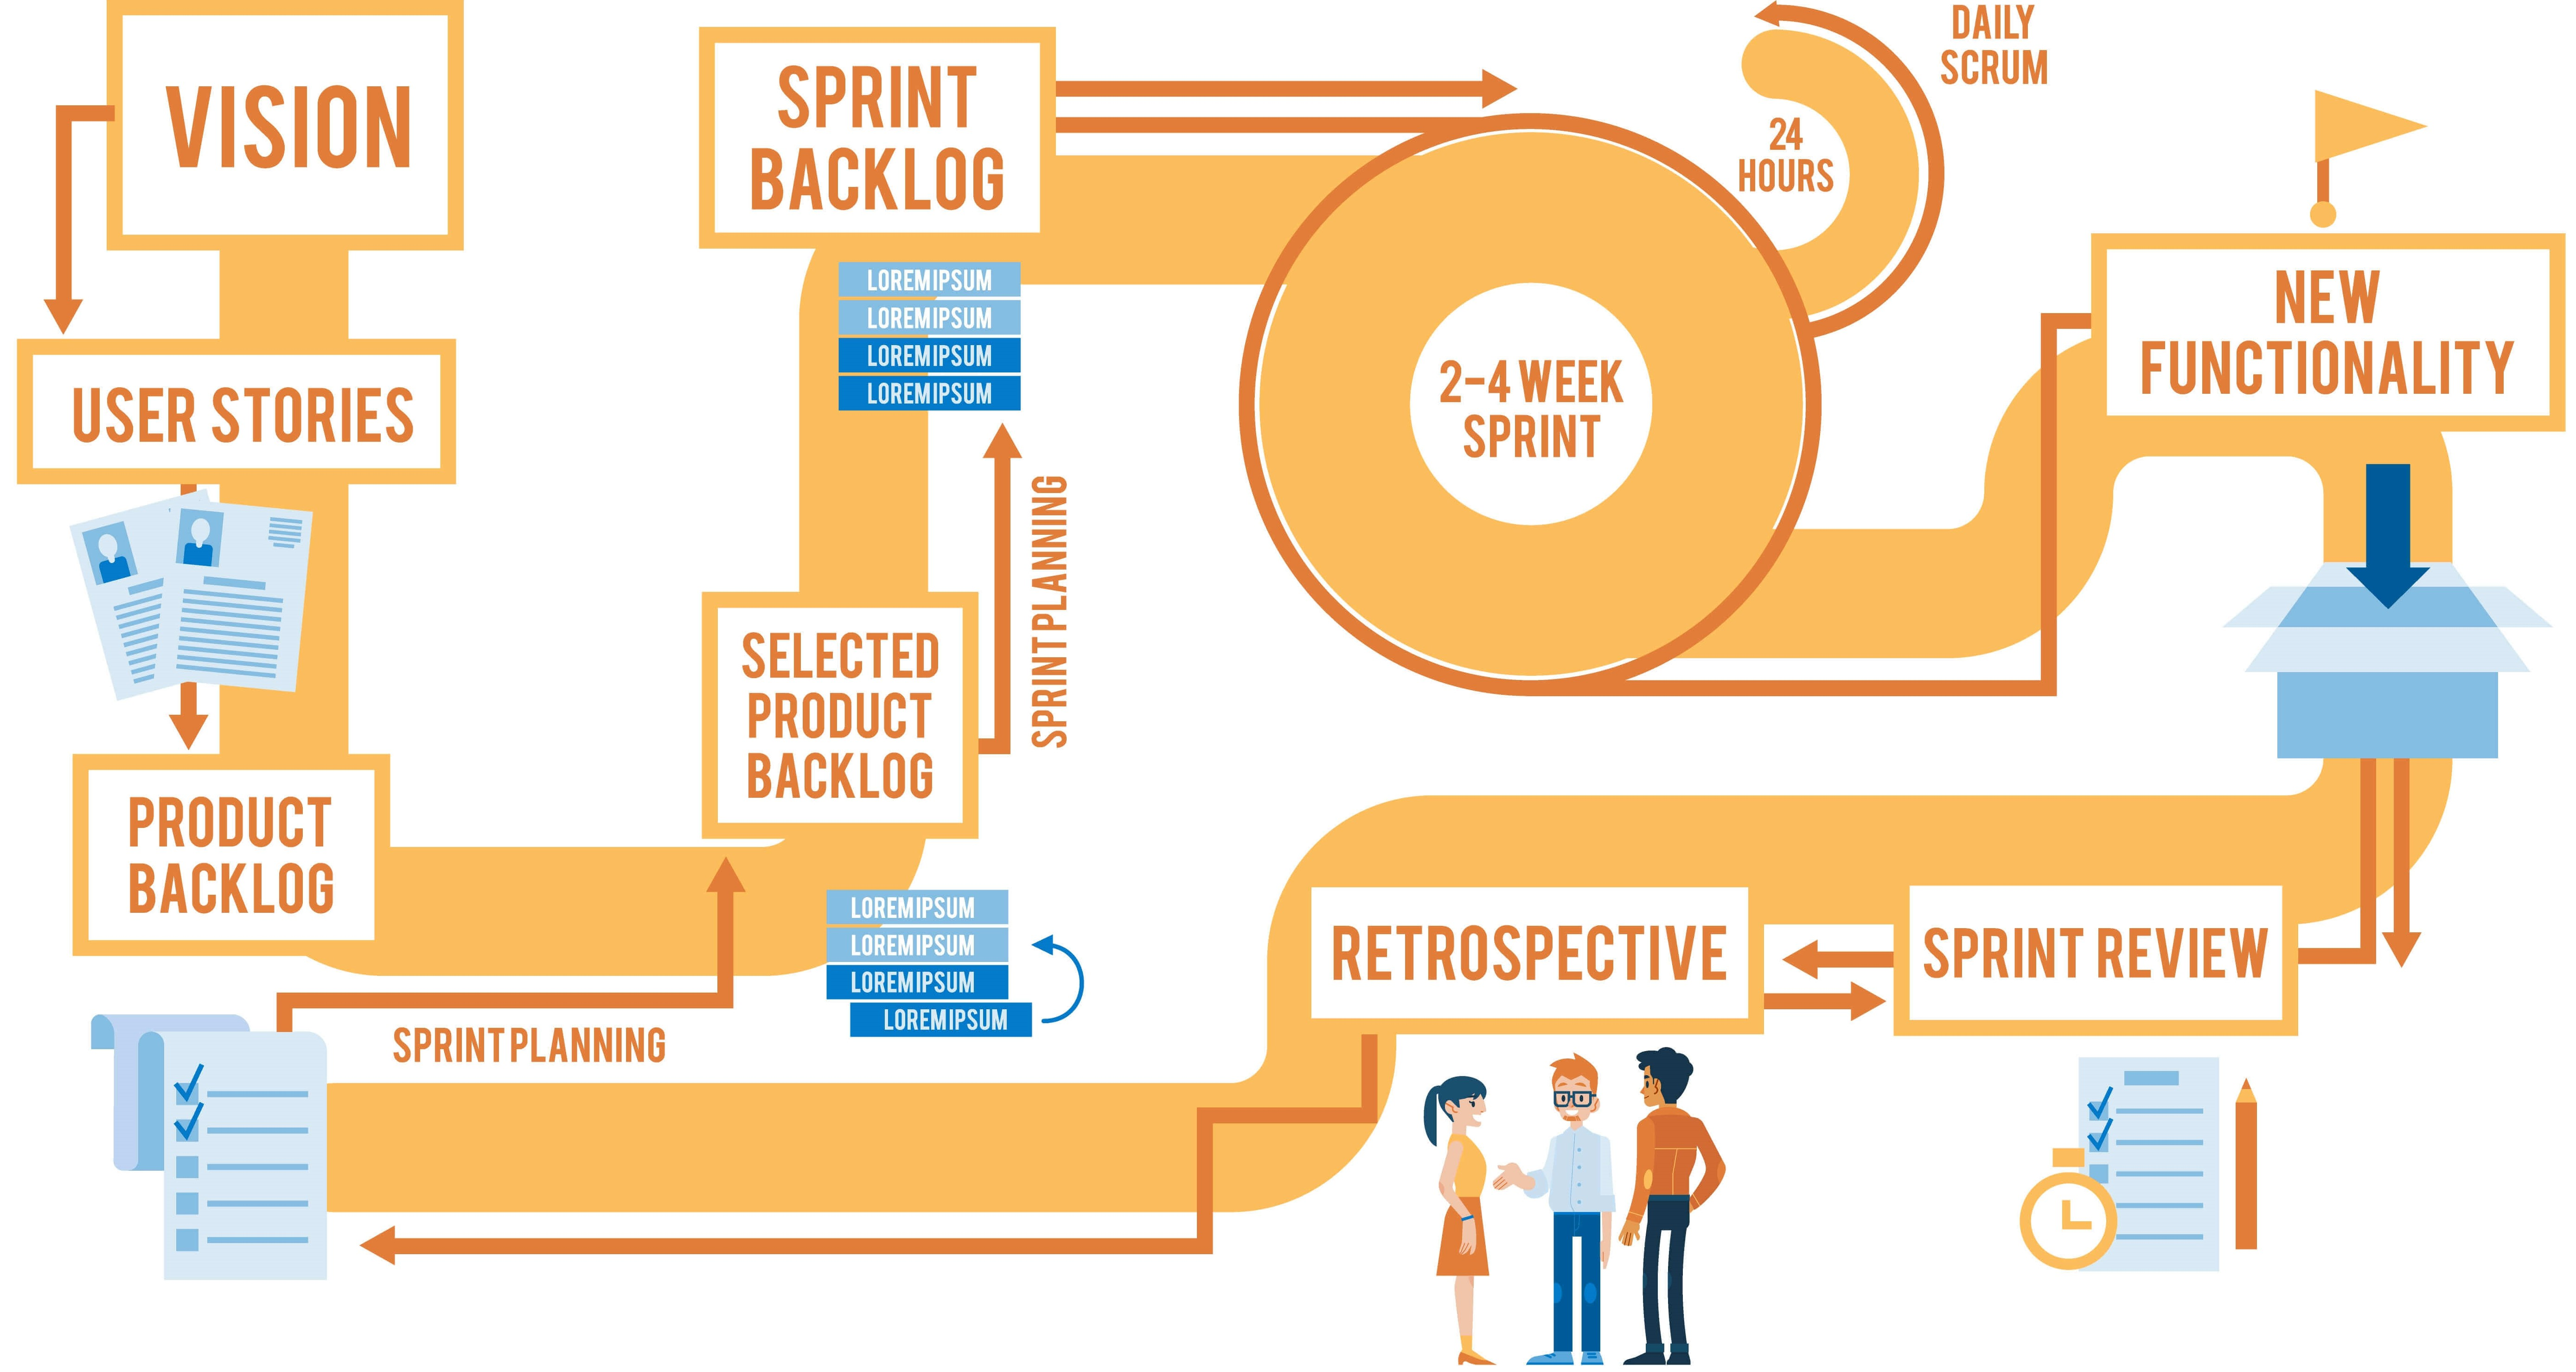
\includegraphics[scale = 0.08]{template/images/scrum.jpg}
    \caption{Il framework Scrum}
    \label{fig:2.1} % Etichetta per il riferimento
\end{figure}